\chapter{Implementation}
This chapter discusses in detail the design and implementation of the functionalities of the programmable switch. First, I describe different design architectures and why a particular architecture is chosen (\S\ref{sec:arch-design}). Then, I move on to explain the P4 implementation of the core logic of the switch (\S\ref{sec:sw}). Lastly, I discuss the additional Verilog components needed to implement the design in hardware (\S\ref{sec:hw}). A repository overview is also given in Appendix \ref{sec:repo}.

\section{System Architecture}
\label{sec:arch-design}
Following the preparation stage, the first objective is to design the system architecture for the switch. The P4 program will then use the architecture as a reference to implement the core logic, making adjustments to the design where necessary.

\subsection{Network Level}
\begin{figure}[!h]
	\centering
	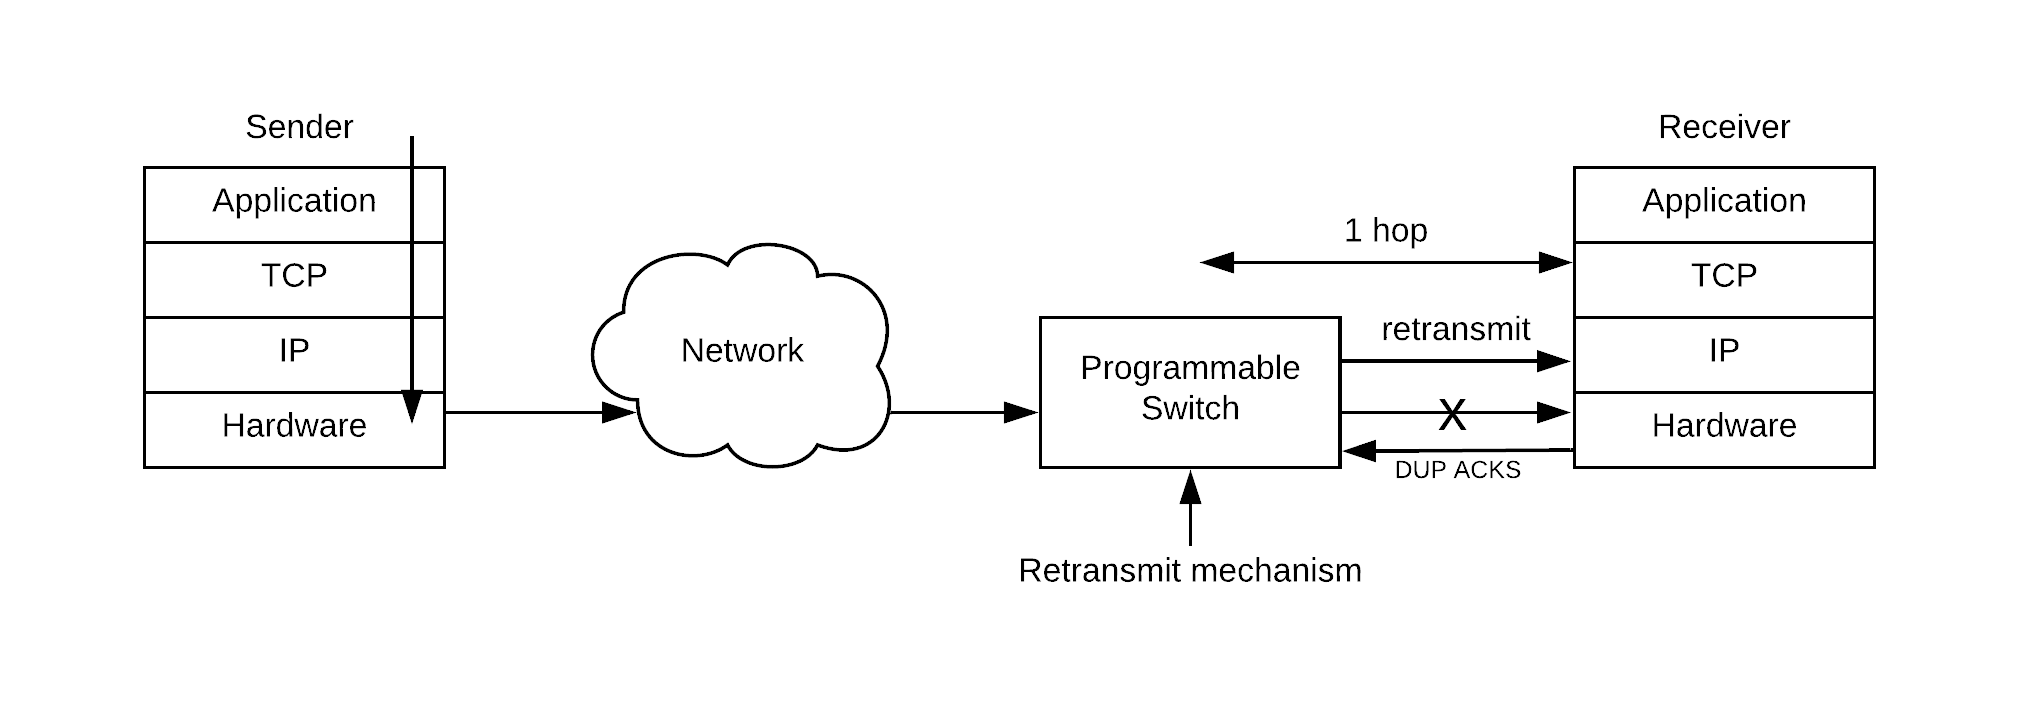
\includegraphics[width=\textwidth]{network.png}
	\caption{The network-level view of the programmable switch. It will be located at the last hop before the receiver, and only performs the fast retransmit on packets from latency-sensitive applications, which are identified by their flow identifier.}
	\label{fig:network}
\end{figure}

To mitigate last-hop drops that are not caused by congestion, the switch will embed the TCP fast retransmit mechanism and will be located in the Top of Rack (ToR) switch (one hop away from the receiver) and not the spine switch (in the core of the network), as illustrated in Figure \ref{fig:network}. Since the switch is programmable, it will be configured to buffer only packets from latency-sensitive high priority applications, identified by their unique \textbf{flow identifier}, while transmitting other packets normally. This design avoids introducing unnecessary buffering of packets of other flows which is the cause of bufferbloat.

\subsection{System Level}
The initial design followed the NetFPGA reference switch design architecture (Figure \ref{fig:ref-switch}), in which the SimpleSumeSwitch module will embed the buffering logic of the switch. When a packet arrives, the switch computes its unique flow identifier from the 5-tuple (IP address pair, Layer 4 port pair and the protocol, which is TCP in this project). If the flow identifier matches the set of pre-defined flows of interest, it will buffer the packet to retransmit. We use a hash table to map flow identifier to another hash table with the packet sequence number as the key and the packet itself as the value. If the packet is an ACK packet, the switch checks if it is a new ACK and updates relevant counters. If it is a DUP ACK, it increments the ACK counter and retransmits if 3 DUP ACKs are received. Figure \ref{fig:flowchart} presents the flowchart showing the buffering logic of this design, with the steps that involve a hash table highlighted in red box.

\begin{figure}[!h]
	\centering
	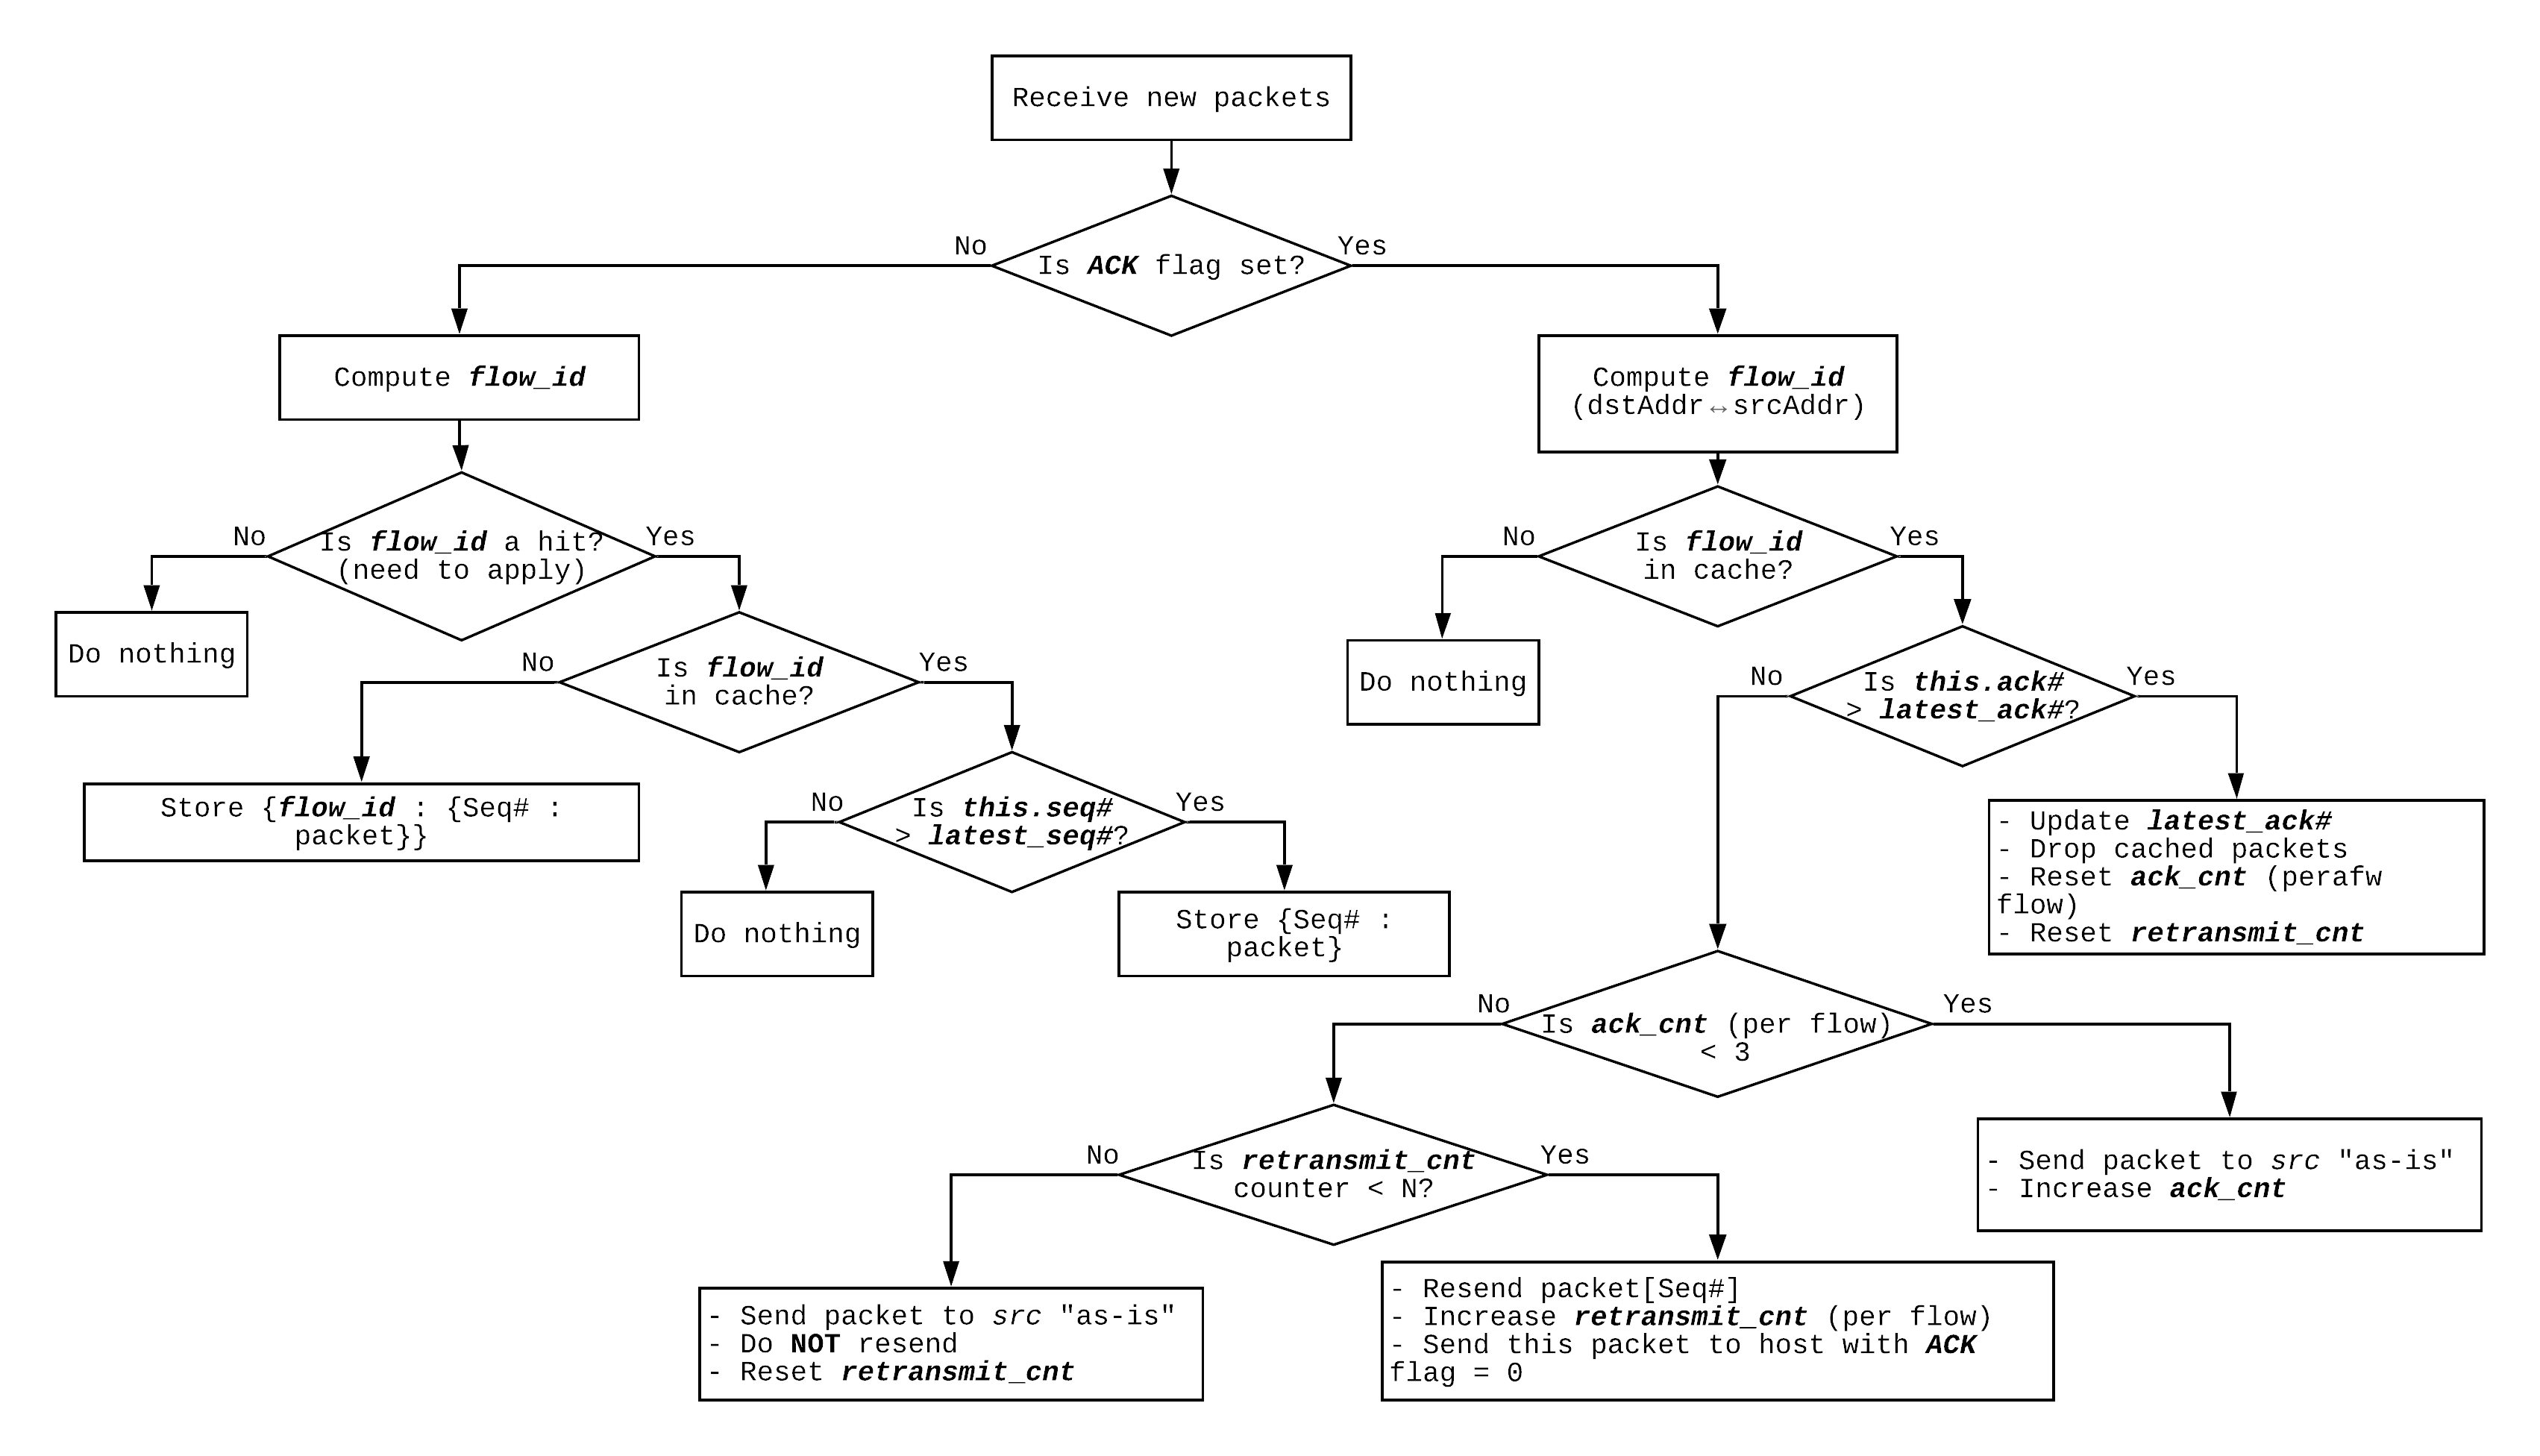
\includegraphics[width=\textwidth]{flowchart.png}
	\caption{Flowchart of the packet retransmit logic. The steps in red box require the ability to store the packet payload.}
	\label{fig:flowchart}
\end{figure}

However, this design did not work due to the limitations of SDNet and the SimpleSumeSwitch architecture of the NetFPGA platform. The SimpleSumeSwitch architecture only supports programmable packet processing without deep packet inspection, i.e. operations on packet headers only. This means that the P4 program would not be able to access the packet payload to store it in the second hash table. Hence, this design cannot be fully expressed in P4 alone.

After careful study of the initial design and the limitations of the platform, I improved my design by adding an additional HDL module that follows the SimpleSumeSwitch module in the original NetFPGA reference switch pipeline (Figure \ref{fig:ref-switch}). The additional module is called the \textit{Cache Queue} and it will buffer packets to be retransmitted. The buffering logic remains largely similar to what was discuss previously. This addresses the issue of P4 programs being unable to access the packet payload. Our reference switch pipeline will now look like Figure \ref{fig:modified-design}. In this new pipeline, when a packet exits the SimpleSumeSwitch module, it will be duplicated and buffered in both the output queue and the cache queue. While the output queue sends the packet to the output ports as soon as it can, the cache queue will hold on to the packet. Once there is a ``signal'' from another packet, the cache queue will drop or send the packet to the output accordingly. The role of the Output Arbiter is similar to that of the Input Arbiter---merging multiple input streams into one output stream---albeit having different names. Section \ref{sec:hw} will explain the implementations of both the Cache Queue and the Output Arbiter in more detail.

\begin{figure}[!h]
	\centering
	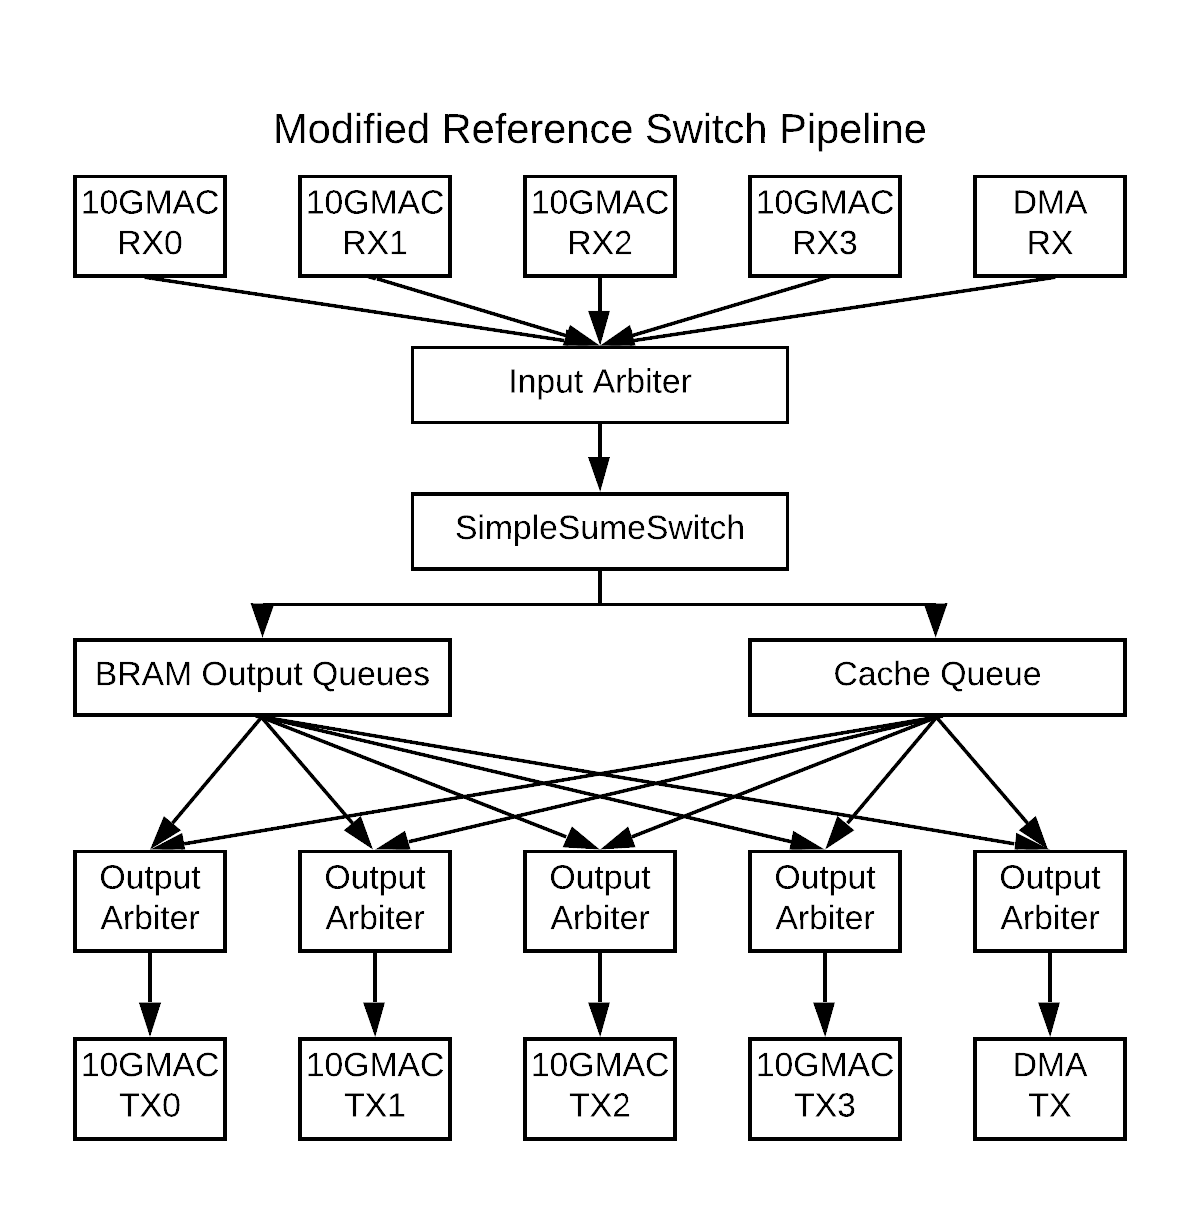
\includegraphics[width=0.5\textwidth]{modified-design.png}
	\caption{Block diagram of the modified reference switch pipeline. Packets are duplicated after the SimpleSumeSwitch module and being buffered in the Cache Queue. Red blocks represent additional modules. Blue blocks represent modules from the reference switch design that are modified.}
	\label{fig:modified-design}
\end{figure}

\section{P4 Implementation}
\label{sec:sw}
As previous introduced in \S\ref{sec:p4-netfpga}, our P4 program follows the SimpleSumeSwitch architecture which consists of a parser, a match-action pipeline, and a deparser, shown in Figure \ref{sss}.

\subsection{The Parser}
Parsers are functions that are responsible for extracting headers out of an incoming packet, written in a state machine style \cite{p4spec}. We can declare a parser with the following code sequence:

{\renewcommand{\baselinestretch}{0.8}\small
	\begin{verbatim}
  // Parser Implementation
  @Xilinx_MaxPacketRegion(1024)
  parser TopParser(packet_in b, 
                  out Parsed_packet p, 
                  out user_metadata_t user_metadata,
                  out digest_data_t digest_data,
                  inout sume_metadata_t sume_metadata);
	\end{verbatim}
}
where \texttt{@Xilinx\_MaxPacketRegion} is Xilinx P4-SDNet's additional annotation for parser/deparser that declares the largest packet size (in bits) the parser/deparser needs to support.
 
Figure \ref{fig:general-fsm} illustrates the general structure of a parser state machine, which includes three predefined states: 
\begin{itemize}[leftmargin=*, noitemsep]
	\item \texttt{start} -- the start state.
	\item \texttt{accept} -- indicating successful parsing.
	\item \texttt{reject} -- indicating a parsing failure.
\end{itemize}
and other internal states that may be defined by the user. Parsers always start in the \texttt{start} state, execute one or more statements, then make a transition to the next state until reaching either the \texttt{accept} or \texttt{reject} states, which are distinct from the user-defined states and are logically outside of the parser. 


\begin{figure}[!h]
	\begin{minipage}{.48\textwidth}
		\centering
		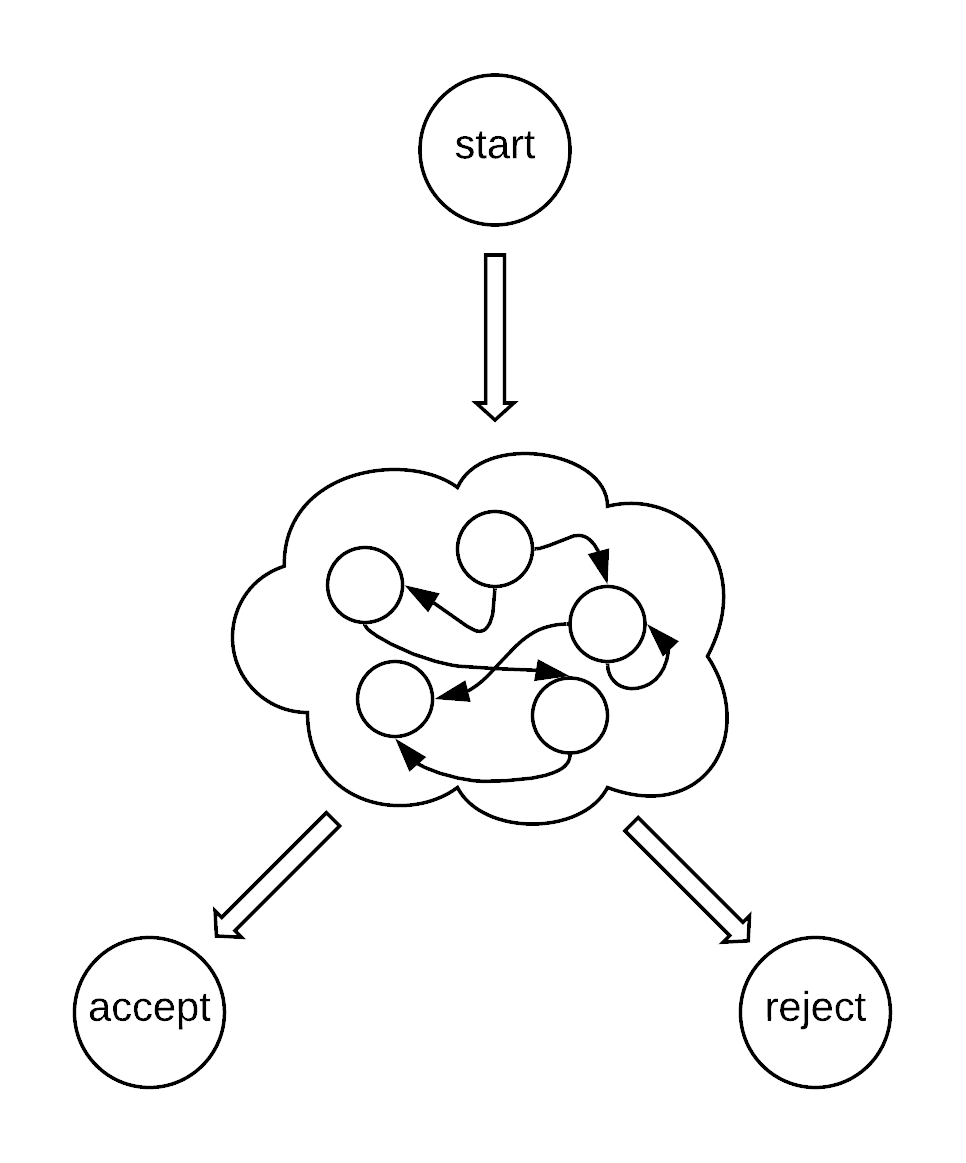
\includegraphics[width=0.7\textwidth]{general-fsm.png}
		\caption{The general state machine structure of a parser.}
		\label{fig:general-fsm}
	\end{minipage}
	\hfill
	\begin{minipage}{.48\textwidth}
		\centering
		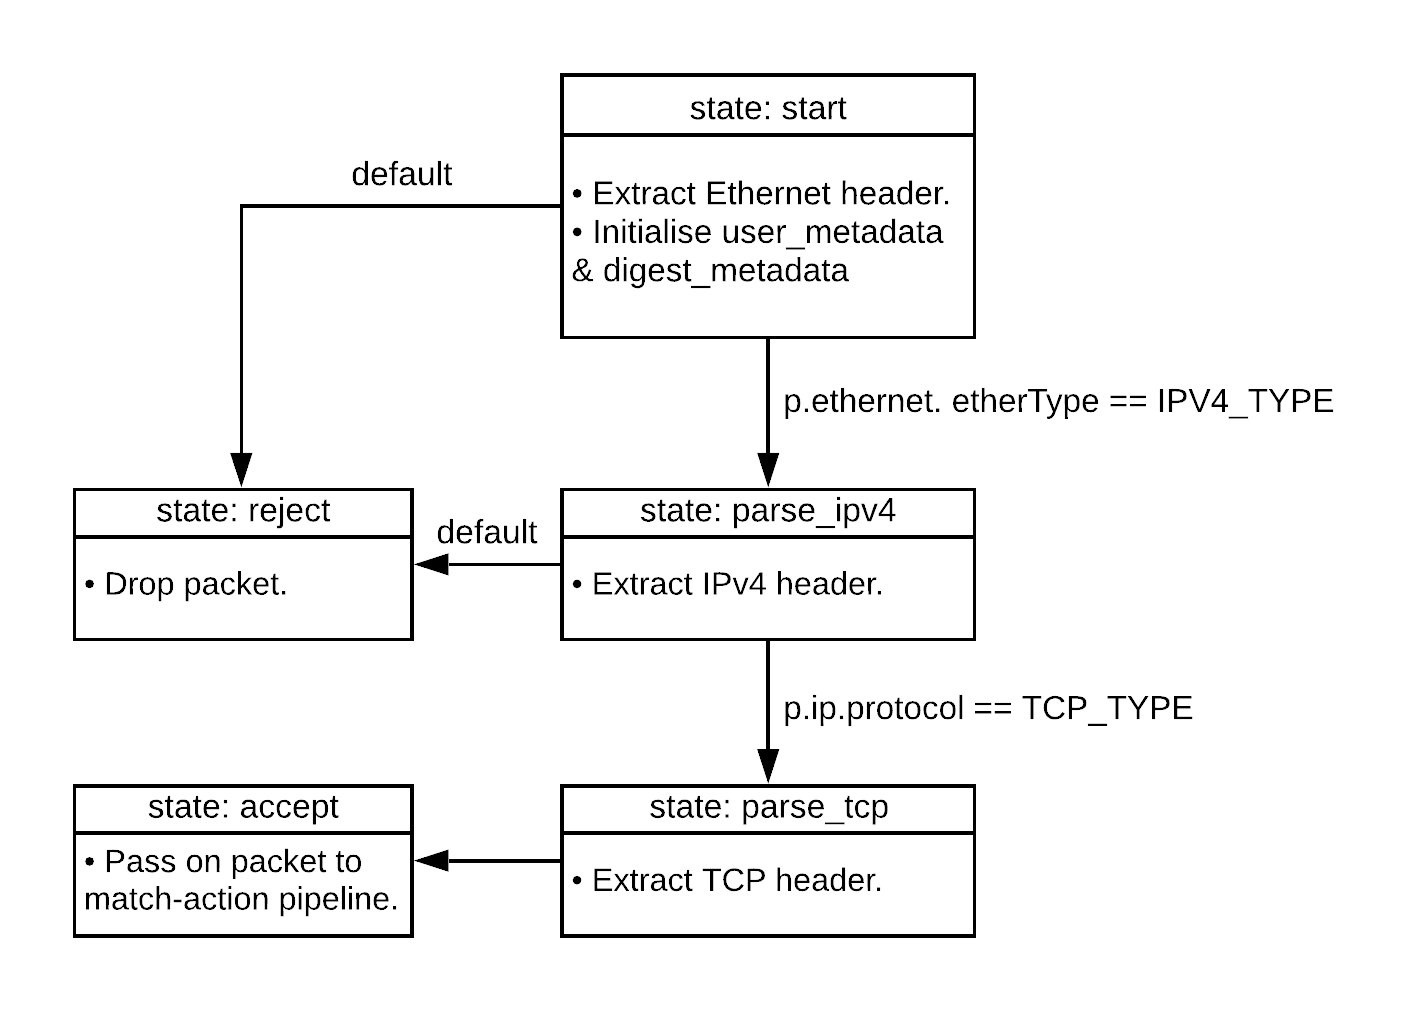
\includegraphics[width=\textwidth]{design-fsm.png}
		\caption{The state machine of the design.}
		\label{fig:design-fsm}
		\vspace{-2em}
	\end{minipage}
\end{figure}

An architecture must specify the behaviour when the \texttt{accept} and \texttt{reject} states are reached. For example, an architecture may specify that all packets reaching the \texttt{reject} state are dropped without further processing. Alternatively, it may specify that such packets are passed to the next block after the parser, with intrinsic metadata indicating that the parser reached the \texttt{reject} state, along with the error recorded. The SimpleSumeSwitch architecture users the SDNet which does not support \texttt{reject}. Hence, the \texttt{reject} state is manually defined and implemented to drop all packets without further processing.

Figure \ref{fig:design-fsm} describes the state machine structure of our parser, which includes a \texttt{start} state (Figure \ref{fig:start}) and two additional user-defined states \texttt{parse\_ipv4} (Figure \ref{fig:parseipv4}) and \texttt{parse\_tcp} (Figure \ref{fig:parsetcp}). The P4 \texttt{select} statement is used to branch in a parser. It is similar to \texttt{case} statement in C or Java, but without ``fall-through behaviour''---i.e., \texttt{break} statements are not needed. Here, our parser first uses the \verb|packet_in| object's \texttt{extract} method to fill out the fields of the Ethernet header. It also initialises the values of the \verb|user_metadata|'s field \verb|digest_data|'s fields to 0. It then transitions to either the \verb|parse_ipv4| state or the \texttt{reject} state based on the value of the Ethernet header’s \texttt{etherType} field. In the \texttt{parse\_ipv4} state, the parser extracts the packet's IPv4 header, looks at its \texttt{protocol} field and transitions to the \texttt{parse\_tcp} state only if it is \texttt{TCP\_TYPE} which is defined to be 6. Otherwise, the packet is rejected. Finally, in the \texttt{parse\_tcp} state, the parser simply extracts the TCP header and then transitions to the \texttt{accept} state, where the packet will be passed to the match-action pipeline. A \texttt{parse\_ethernet} state could be defined similarly to \verb|parse_ipv4| and \verb|parse_tcp|, but I decided to include the parsing of the Ethernet header within the \texttt{start} state, together with initialising the metadata, for simplicity.

\begin{figure}[!h]
	{\renewcommand{\baselinestretch}{0.8}\small
		\begin{verbatim}
   state start {
     b.extract(p.ethernet);
     user_metadata.unused = 0;
     digest_data.unused = 0;
     digest_data.flow_id = 0;
     digest_data.tuser = 0;
     transition select(p.ethernet.etherType) {
       IPV4_TYPE: parse_ipv4;
       default: reject;
     } 
   }
		\end{verbatim}
	}
\caption{The definition of \texttt{start} state.}
\label{fig:start}
\end{figure}

\begin{figure}[!h]
	\begin{minipage}{.48\textwidth}
		{\renewcommand{\baselinestretch}{0.8}\small
		\begin{verbatim}
		state parse_ipv4 {
		  b.extract(p.ip);
		  transition select(p.ip.protocol) {
		    TCP_TYPE: parse_tcp;
		    default: reject;
		  }
		}
		\end{verbatim}
		}
 		\caption{The definition of \texttt{parse\_ipv4} state.}
 		\label{fig:parseipv4}
	\end{minipage}
	\hfill
	\begin{minipage}{.48\textwidth}
		{\renewcommand{\baselinestretch}{0.8}\small
		\begin{verbatim}
		state parse_tcp {
		  b.extract(p.tcp);
		  transition accept;
		}
		    
		    
		    
		\end{verbatim}
		}	
		\caption{The definition of \texttt{parse\_tcp} state.}
		\label{fig:parsetcp}
	\end{minipage}
\end{figure}
		
	\subsection{The Match-Action Pipeline}
A match-action pipeline is a control block where the match-action packet processing logic is implemented. A match-action pipeline uses \textit{tables}, \textit{actions}, and \textit{imperative code} (indicated by the \textbf{\texttt{control}} keyword) to manipulate input headers and metadata \cite{fpga19}. This match-action processing model was originally introduced as the core around which the OpenFlow model for SDN was built \cite{mckeown}. Our match-action pipeline can be defined by the following code sequence:

{\renewcommand{\baselinestretch}{0.8}\small
	\begin{verbatim}
  // Match-action pipeline
  control TopPipe(inout Parsed_packet p,
                inout sume_metadata_t sume_metadata, 
                inout digest_data_t digest_data, 
                inout user_metadata_t user_metadata) {
    /** actions **/
    /** tables **/
    /** logic **/          
  }
	\end{verbatim}
}

This pipeline receives four inputs: the parsed packet \texttt{p}, the SUME metadata, the digest data and the user metadata. The direction \texttt{inout} indicates that the parameters are both an input and an output. Thus, their values, including the fields in the headers of packet \texttt{p}, can be modified. Nonetheless, the \verb|user_metadata| field was not used in this design.

When we defines a match-action table (using the P4 \textbf{\texttt{table}} keyword), we declare various properties such as the header and/or metadata field(s) to match upon, the type of match to be performed, a list of all possible actions that can be invoked, the number of entries to allocate for the table, and a default action to invoke if no match is found. A table entry contains a specific key to match on, a \textit{single} action to invoke when the entry produces a match, and any data to provide to the action when it is invoked. The table entries are populated at runtime by the control plane software.

\begin{figure}[!h]
	\centering
	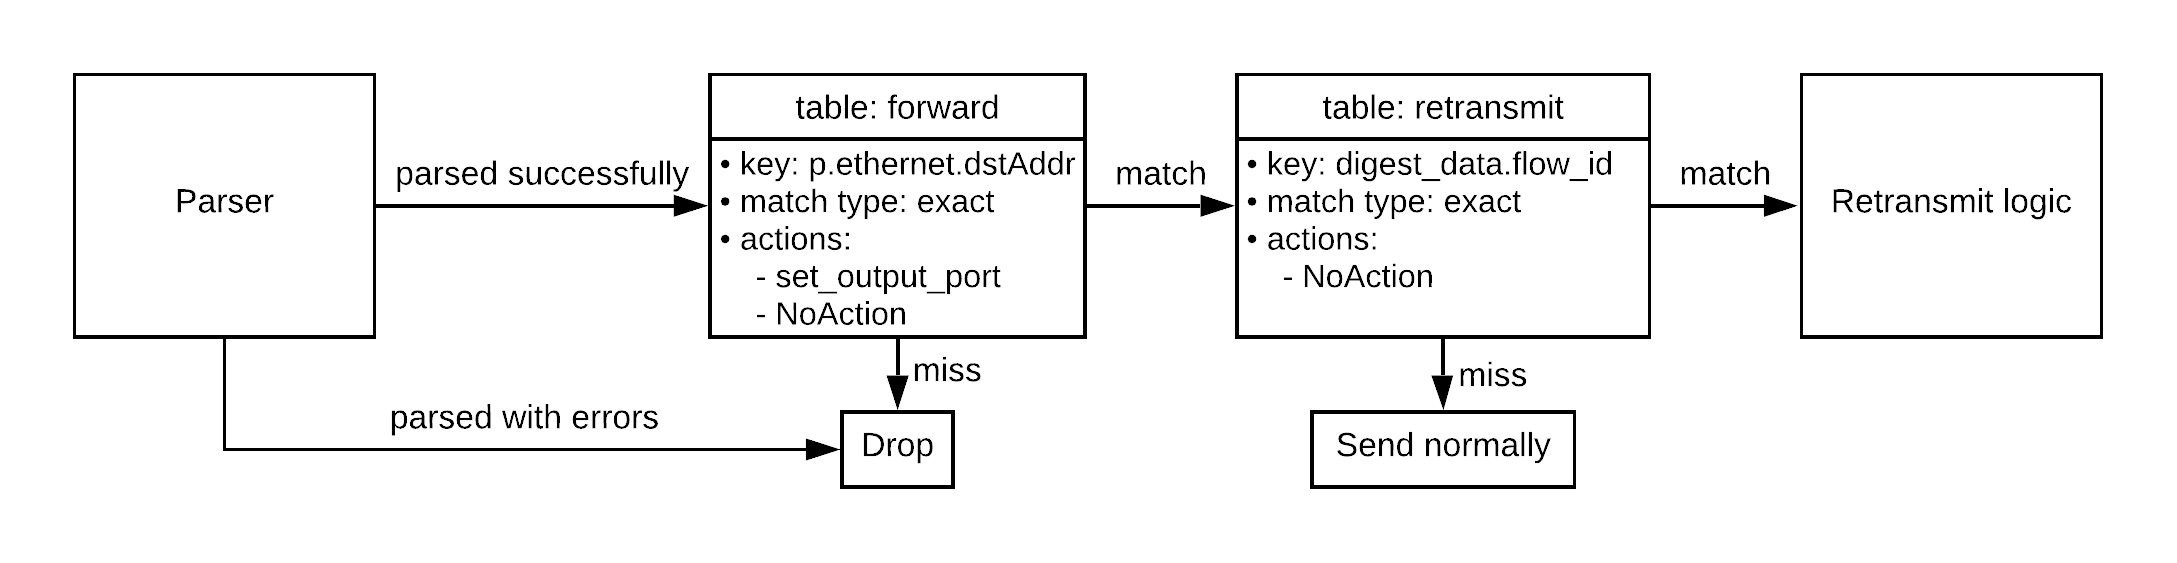
\includegraphics[width=\textwidth]{mapipe.png}
	\caption{The packet processing program of the switch. Incoming packets will go through a parser, a match-action pipeline, which including the buffereing logic and a deparser, before coming out to the output queue and the cache queue.}
	\label{fig:mapipe}
\end{figure}

\begin{table}[!h]
	\centering
	\caption{Entries for the \texttt{forward} table.}
	\label{tab:forward}
	\begin{tabular}{ | c | c | c |}
		\hline
		\textbf{Key} & \textbf{Action} & \textbf{Action Data} \\ \hline
		08:11:11:11:11:08 & \verb|set_output_port| & 0b00000001 \\ \hline
		08:22:22:22:22:08 & \verb|set_output_port| & 0b00000100 \\ \hline
		08:33:33:33:33:08 & \verb|set_output_port| & 0b00010000 \\ \hline
		08:44:44:44:44:08 & \verb|set_output_port| & 0b01000000 \\ \hline
		ff:ff:ff:ff:ff:ff & \verb|set_output_port| & 0b01010101 \\ \hline
	\end{tabular}
\vspace{2em}
	\centering
	\caption{Entries for the \texttt{retransmit} table.}
	\label{tab:retransmit}
	\begin{tabular}{ | c | c | c |}
		\hline
		\textbf{Key} & \textbf{Action} & \textbf{Action Data} \\ \hline
		\texttt{792281630049477301766976897099}  & NoAction & \_ \\ \hline
	\end{tabular}
\end{table}

Figure \ref{fig:mapipe} illustrates the control flow program acting on a packet going through our match-action pipeline, which comprises two match-action tables: \texttt{forward} and \texttt{retransmit}. The \verb|forward| table (Table \ref{tab:forward}) uses the Ethernet destination address to determine the output port for the next hop. For instance, if the destination MAC address is \verb|08:11:11:11:11:08|, the output port will be set to \verb|nf0| (the first port). If the destination address is \verb|08:22:22:22:22:08|, the output port will be set to the second port \verb|nf1|, and so on. If this lookup fails, the packet is broadcasted to all ports except for the source port by xor-ing the source port with \verb|0b01010101|: \verb|sume_metadata.dst_port = 0b01010101^sume_metadata.src_port|. 

The \verb|retransmit| table (Table \ref{tab:retransmit}) checks the computed flow identifier of the packet, which is stored in the \texttt{digest\_data.flow\_id} field: if it matches our flow of interest, the packet will be monitored to assist the TCP fast retransmit process. Otherwise, the packet will just be delivered normally. This allows us to specify the set of flows from latency-sensitive applications by adding their unique flow identifier to the table, in decimal representation. The key in Table \ref{tab:retransmit} represents---in decimal---the 104-bit flow identifier of a flow from IP address \verb|10.0.0.1| port \verb|55| to IP address \verb|10.0.0.2| port \verb|75|. Since the retransmit logic is complicated and cannot be expressed using a single action, no action is taken if there is a match, hence no action data is provided. Instead, the packet will be inspected more carefully through a series of actions.

In our match-action pipeline, the following actions were defined: \texttt{set\_output\_port} sets the output port on the SUME board for packets whose Ethernet destination address matches what was defined in the \verb|forward| table; \texttt{compute\_flow\_id} computes the flow identifier of the packet to look up in the \verb|retransmit| table; \texttt{cache\_write}, \texttt{cache\_read} and \texttt{cache\_drop} modify \texttt{digest\_data.tuser} to signal the cache queue to cache, retransmit and drop the packet at the head of the queue respectively.

	\subsection{The Extern Functions}
	\label{sec:extern}
P4 extern functions, or externs, are device-specific functions that are not described in the core P4 language---a kind of ``black boxes'' for P4 programs \cite{ibanez}. On NetFPGA, extern functions are implemented in HDL (Verilog). In other environments, they can be defined in any language, e.g. C++. The P4 program just sees the inputs and outputs, as parameters and results. There are two types of extern functions: stateless (reinitialised for each packet) and stateful (keeping states between packets). The stateful atomic externs are inspired by the Domino atoms \cite{domino}. P4$\rightarrow$NetFPGA provides a set of commonly-used extern functions, shown in Table \ref{tab:externs}. 

An extern function can be declared using the syntax

{\renewcommand{\baselinestretch}{0.8}\small
	\centering
	\begin{verbatim}
  extern void <name>_<extern_type>(in T1 data1,in T2 data2,...,out D result);
	\end{verbatim}
} 

The following code sequence shows an example of declaring a simple longitudinal redundancy check hash extern:

{\renewcommand{\baselinestretch}{0.8}\small
	\begin{verbatim}
  @Xilinx_MaxLatency(1)
  @Xilinx_ControlWidth(0)
  extern void hash_lrc(in T in_data, out D result);
	\end{verbatim}
}
where \texttt{@Xilinx\_MaxLatency} and \texttt{@Xilinx\_ControlWidth} are Xilinx P4-SDNet's additional annotations to allow P4 programmer to specify the number of clock cycles to complete the extern operation, and the width of the address space allocated to this register respectively. The control width should always be equal to the width of the index field so that the control plane can access all register entries.

Using the retransmit logic in Figure \ref{fig:flowchart} as the reference, I defined the following externs based on the externs template provided by P4$\rightarrow$NetFPGA:
\begin{itemize}[leftmargin=*, noitemsep]
	\item \verb|hash_lrc|: similar to P4$\rightarrow$NetFPGA's LRC hash function, this splits the input data into multiple words and \textit{XOR} each word together to obtain the result. This is used to hash the flow identifier of the packet. The hash result is used to index into the registers which store the counters for that particular flow.
	\item \verb|seq_no_reg_praw|: stores the latest sequence number that the switch has seen from the sender. This is updated when a new packet is received.
	\item \verb|latest_ack_no_reg_praw|: stores the latest acknowledgement number from the receiver. This is updated when a new ACK packet is received.
	\item \verb|pkts_cached_cnt_reg_raw|: stores the number of packets that the cache queue is buffering. This is updated when a new packet is buffered, or when some packets are read or dropped from the cache queue. When the latter happens, the value in the register is decremented either by 1 (read) or a positive value (dropped). The number of cached packets to drop is calculated by \verb|(pkt.tcp.ackNo-latest_result) >> PKT_SIZE|. This limits the design to only be able to handle a single packet size that is configured in the P4 code. \textbf{For the purpose of easier debugging and testing process, I defined the packet size to be 64B}.
	\item \verb|ack_cnt_reg_praw|: stores the number of duplicate acknowledgements. This is updated when the switch received a duplicate acknowledgement, that is when \verb|pkt.tcp.ackNo == latest_ack_no|. When the value of the counter reaches 2, the third duplicate acknowledgement will signal the cache queue, via \verb|digest_data.tuser|, to retransmit the packet with the sequence number in the DUP ACK packet. This packet will also be sent back to the sender with its ACK flag set to 0. This is because we do not want the sender to retransmit the packet, so an ACK flag of 0 keeps the counter of the sender at 2.
	\item \verb|retransmit_cnt_reg_ifElseRaw|: stores the number of times of the DUP ACK packet has been retransmitted. Once a retransmission occurs, this counter will be set to 1. Subsequent DUP ACK packets will be sent back to the sender since the switch would now assume that the reason for packet loss is not due to a momentary failure, but rather to true congestion or inability to sustain the data rate.
\end{itemize}

The P4$\rightarrow$NetFPGA \verb|raw|, \verb|praw| and \verb|ifElseRAW| externs, by default, return the values of the register after modification. However, I often want to read the value of the register, \textit{then} modify it. Thus, I changed their implementation so that they return the values before modification by having a temporary variable that stores the current value of the register. I also modified them to include the \verb|SUBTRACT| operation.

Another important feature of P4$\rightarrow$NetFPGA externs is that to guarantee consistency between successive packets, stateful operations cannot be pipelined; each performs an atomic read-modify-write operation per packet in hardware. In other words, each stateful extern can only be accessed \textit{one} time in the P4 code. Multiple calls to the extern function will generate multiple instances of the atom, thus giving unexpected results. To illustrate this difficulty, let us look at an example of using a RAW extern (Read, add to, or overwrite state---Table \ref{tab:externs}) called \verb|curr_seq_no_raw| to store the latest sequence number that the switch has seen. To determine whether an incoming packet is a new packet, one first needs to perform a \verb|READ| operation from the register to get the latest sequence number. If it is indeed a new packet, one then needs to perform a \verb|WRITE| operation to update the value of the latest sequence number stored in the register. We can see, from the pseudocode in Figure \ref{fig:pseudo}, that we have made two calls to the extern \verb|curr_seq_no_raw|, which is not feasible with P4$\rightarrow$NetFPGA externs.

\begin{figure}[!h]
	{\renewcommand{\baselinestretch}{0.8}\small
		\begin{verbatim}
  def check_new_packet(pkt):
    curr_seq_no = curr_seq_no_raw(READ, 0) // READ from the register the 
                                           // current latest sequence number
    if (pkt.seqNo > curr_seq_no):             
      curr_seq_no_raw(WRITE, pkt.tcp.seqNo) // WRITE to the register the new 
                                      // latest sequence number
                                      // Access the extern the SECOND time!!!
      return True
    else:
      return False
		\end{verbatim}
	}
	\caption{Pseudocode for checking whether an incoming packet is a new packet.}
	\label{fig:pseudo}
\end{figure}

This complicates my P4 program significantly since we would naturally require two operations to perform most of the functions in the retransmit logic. Furthermore, some externs need to be called both when the packet is an ACK packet and when it is not, thus inevitably require at least two calls. To circumvent this, I used ``pseudo-parameters'', the PRAW extern (Either perform RAW or do not perform RAW based on predicate---Table \ref{tab:externs}) and the ifElseRAW extern (Two RAWs, one each for when a predicate is true or false---Table \ref{tab:externs}). The actual PRAW extern has eight parameters. For simplicity, let us define a simplified version of the PRAW extern, which has six parameters:
\begin{itemize}[leftmargin=*, noitemsep]
	\item \verb|newVal|: the new value to write into the register.
	\item \verb|operation|: the operation to perform (read, add to or write).
	\item \verb|compVal|: the value to compare to the current value of the register.
	\item \verb|comparator|: the operation used to compare \verb|compVal| to the current value of the register. \verb|compVal| and \verb|comparator| together define the predicate that decides whether or not the register value will be modified. If the predicate is true then the register may be modified, otherwise it will not be. The predicate is defined as: <\verb|compVal|> <\verb|comparator|> <\verb|register_value|>.
	\item \verb|latest_value|: the current value of the register.
	\item \verb|result|: indicates whether or not the predicate was \verb|True| or \verb|False|.
\end{itemize}

Continue from the previous example, our extern to access the register that stores the value of the latest sequence number that the switch has seen has to be called three times: when the packet is an ACK packet, we want to read the latest sequence number to see if the ACK number is the next sequence number; when the packet is not an ACK, we want to read the latest sequence number to determine if the packet is a new packet, and write back the updated latest sequence number if necessary. Now, using the pseudo-parameters, we can perform the three operations using only one call to the \verb|curr_seq_no_praw| extern (Figure \ref{fig:fix}). If the packet is an ACK packet, \verb|seq_no_compVal| is set to 0 and \verb|comparator| is set to \verb|GREATER_THAN|, so the predicate can never be true, since the value of \verb|pkt.seqNo| is non-negative. The value of \verb|latest_seq_no_value| becomes the value of the register after the extern call. Thus, we essentially perform a \verb|READ| operation. On the other hand, if the packet is not an ACK packet, \verb|seq_no_compVal| is set to \verb|pkt.seqNo|, and we now \verb|WRITE| to the register if it is greater than the current latest sequence number. Otherwise, \verb|latest_seq_no_value| contains the value of the register after the extern call, as above. The same technique is used for the ifElseRAW extern.

\begin{figure}[!h]
	{\renewcommand{\baselinestretch}{0.8}\small
		\begin{verbatim}
  def access_sequence_number(pkt):
    result = False
    latest_seq_no_value = 0
    
    if pkt is an ACK pkt:
      operation = WRITE
      seq_no_compVal = 0
      comparator = GREATER_THAN
    else:
      operation = WRITE
      seq_no_compVal = pkt.seqNo
      comparator = GREATER_THAN
    
    // Access the extern ONE time -- OK!
    curr_seq_no_praw(pkt.tcp.seqNo, operation, seq_no_compVal, 
                 comparison, latest_seq_no_value, result);
    
    return (latest_seq_no_value, result)
		\end{verbatim}
	}
	\caption{Pseudocode for using ``pseudo-parameters'' to perform three operations using only one call to the extern.}
	\label{fig:fix}
\end{figure}

With the actions and externs replacing the hash tables, our retransmit logic will now look like Figure \ref{fig:new-flowchart}.

\begin{figure}[!h]
	\centering
	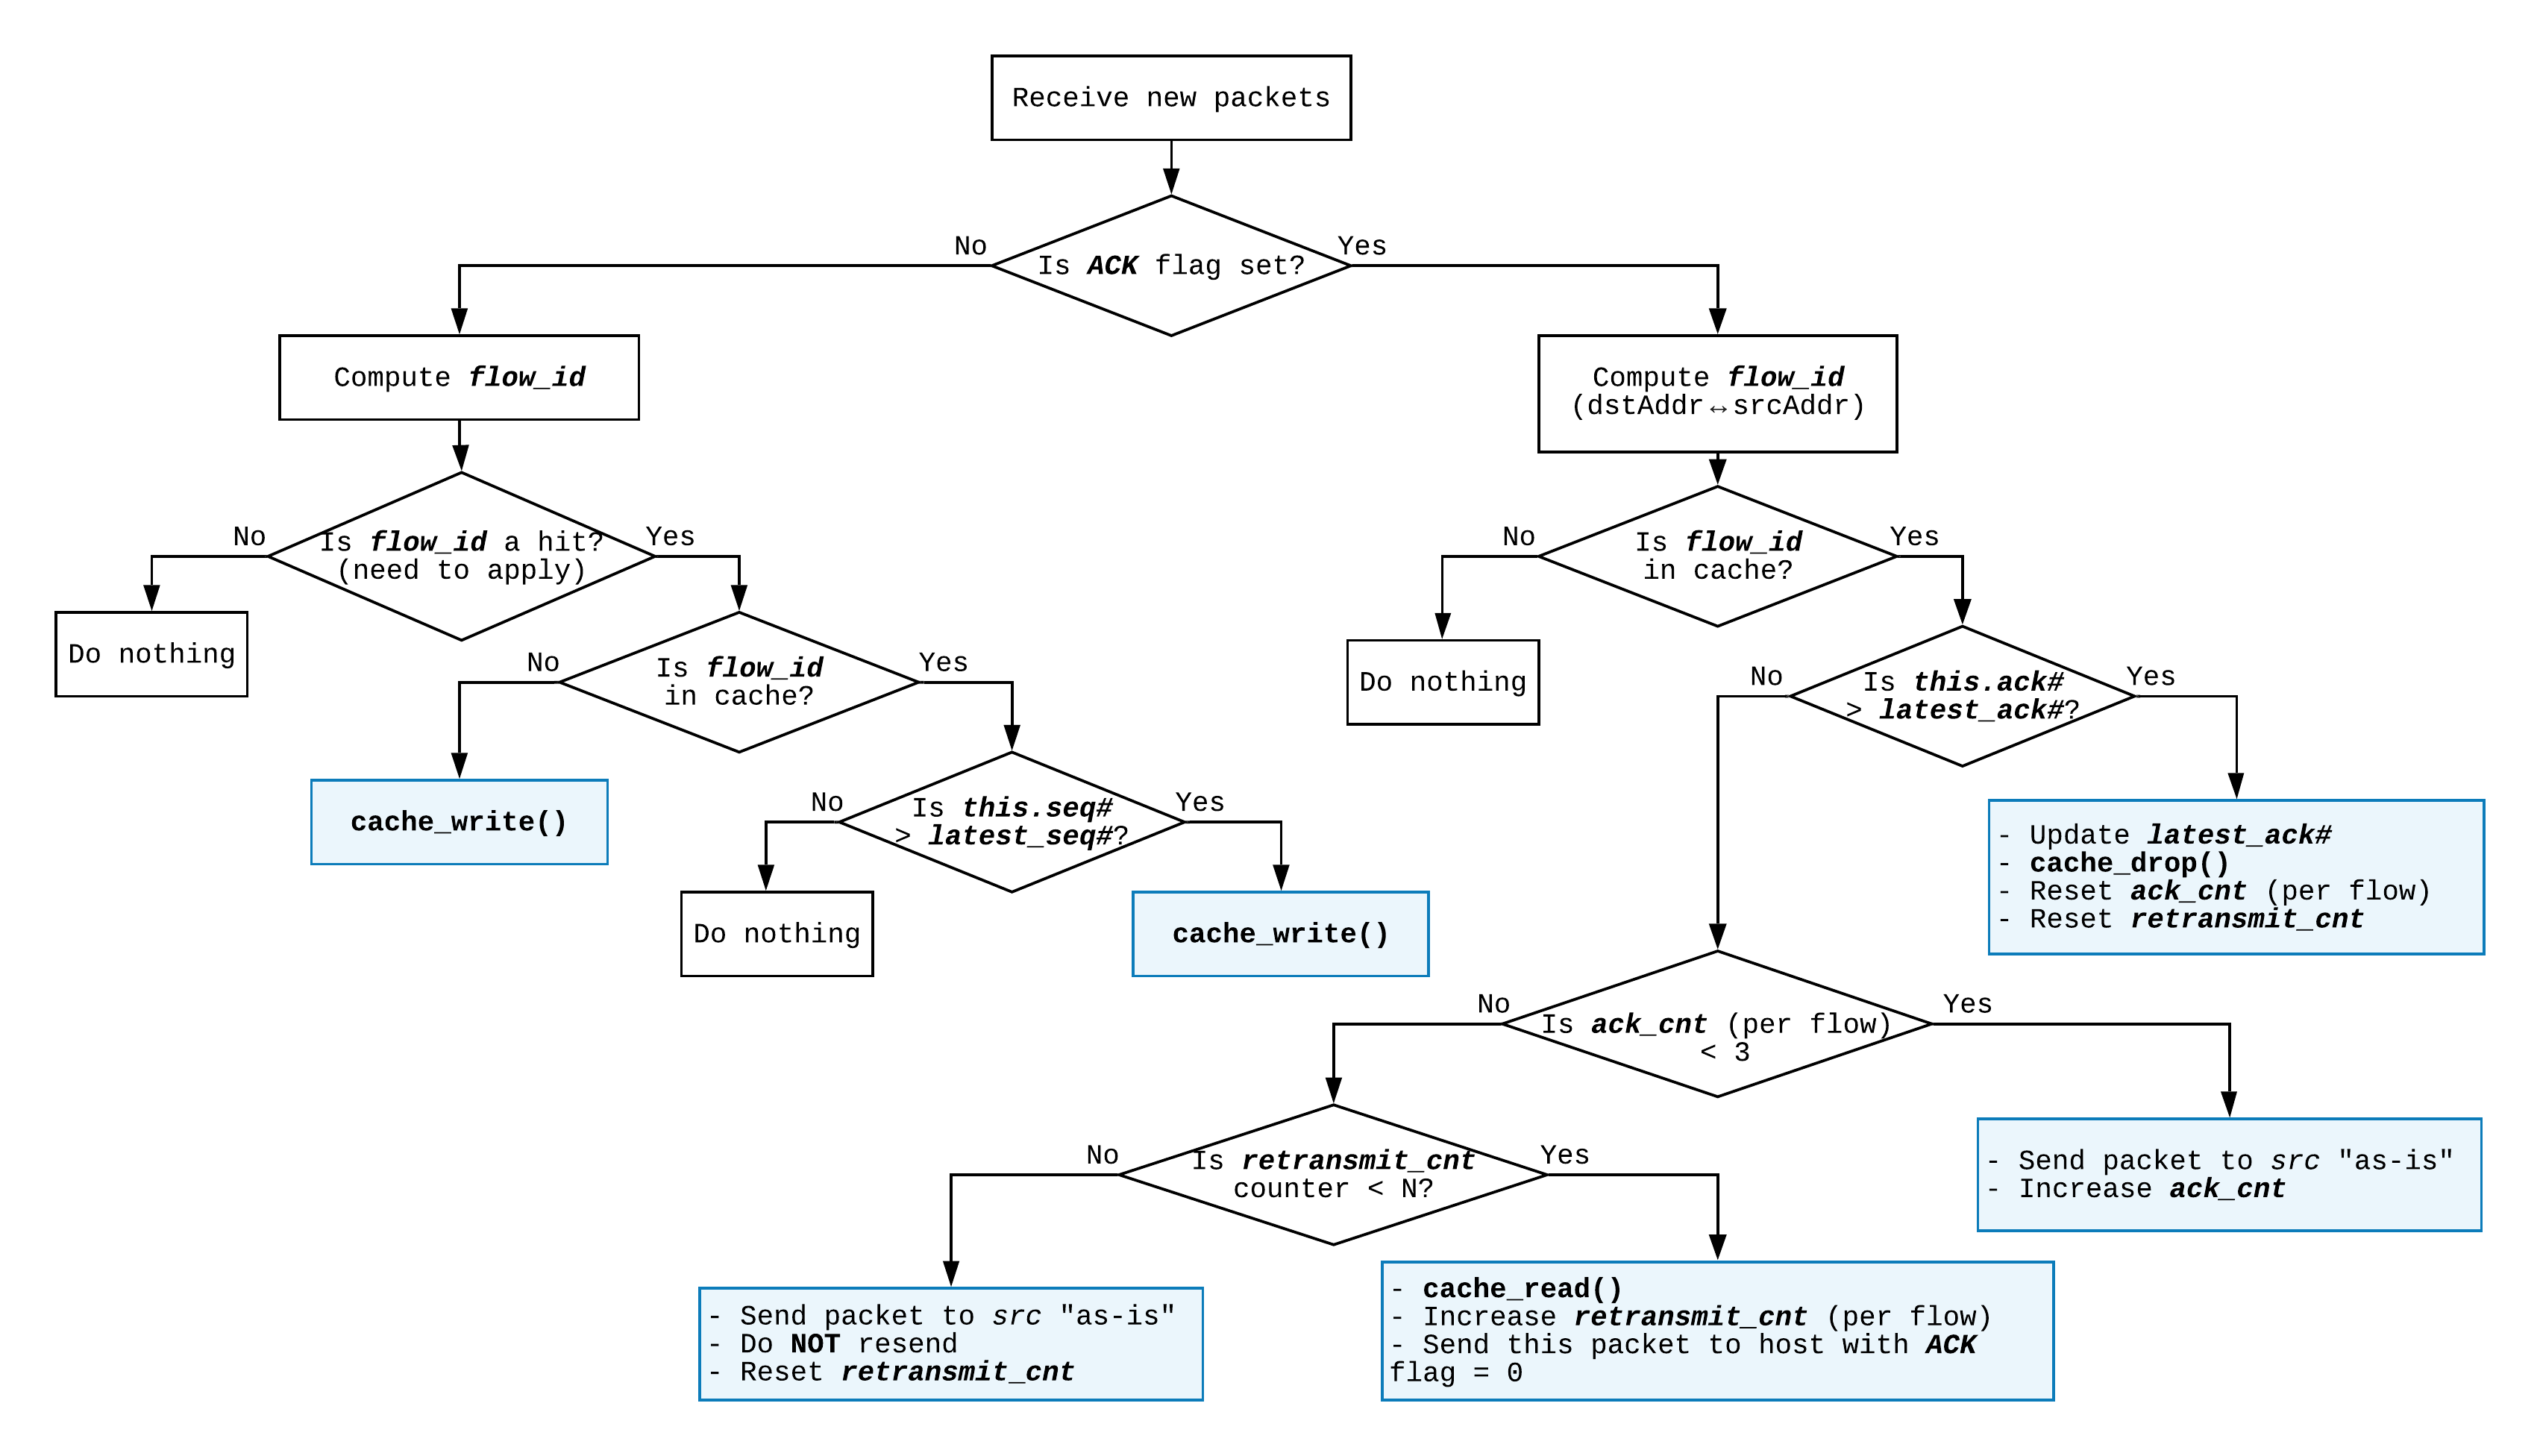
\includegraphics[width=\textwidth]{new-flowchart.png}
	\caption{Flowchart of the packet retransmit logic using actions and externs. The steps involved are highlighted in blue box.}
	\label{fig:new-flowchart}
\end{figure}

	\subsection{The Deparser}
The inverse of parsing is deparsing, or packet assembly, where the outgoing packet is constructed by reassembling the packet headers as computed by the pipeline onto an outgoing packet byte stream. P4 does not provide a separate language for packet deparsing; deparsing is done in a \textbf{\texttt{control}} block that has at least one parameter of type \verb|packet_out| because it only involves sequential logic as used for actions \cite{p4spec}. The advantage of this approach is that it makes deparsing explicit, but decouples it from parsing. 

A header is added to the packet using the \verb|packet_out| object's \texttt{emit} method. The following code block, which implements the deparser of the switch, first writes an Ethernet header, followed by an IPv4 header, and then a TCP header into a \verb|packet_out|. Since emitting a header appends the header to the \verb|packet_out| only if the header is valid, P4 first checks the validity of the headers before serialising them.

{\renewcommand{\baselinestretch}{0.8}\small
\begin{verbatim}
  // Deparser Implementation
  @Xilinx_MaxPacketRegion(8192)
  control TopDeparser(packet_out b,
                  in Parsed_packet p,
                  in user_metadata_t user_metadata,
                  inout digest_data_t digest_data, 
                  inout sume_metadata_t sume_metadata) { 
    apply {
      b.emit(p.ethernet); 
      b.emit(p.ip);
      b.emit(p.tcp);
    }
  }
\end{verbatim}
}

In summary, the switch will perform the following tasks in the SimpleSumeSwitch module:
\begin{enumerate}[label*=\arabic*., leftmargin=*, noitemsep]
	\item Receive and parse packet from the sender. (Parser)
	\item Look up the Ethernet destination address to determine the output port. Broadcast to all but the source port on a miss. (Match-action pipeline)
	\item Compute the flow identifier of the packet. (Match-action pipeline)
	\item Look up the flow identifier of the packet to determine if it should be monitored. Send normally on a miss. (Match-action pipeline)
	\item Set \texttt{digest\_data.tuser} and/or set the \texttt{ACK} flag in the TCP header appropriately. (Match-action pipeline)
	\item Construct the final packet by appending the headers back and send it to the receiver. (Deparser)
\end{enumerate}

\section{Verilog Implementation}
\label{sec:hw}
	\subsection{The Cache Queue}
The cache queue has the basic functionalities similar to those of the output queue of the NetFPGA reference switch design (Figure \ref{fig:ref-switch}): buffer packets from the SimpleSumeSwitch module while they wait to be sent to the output ports. However, since the role of the cache queue is to buffer packets to \textit{retransmit}, we want to be able to signal the cache queue when to buffer a packet, when to drop a packet, when to read a packet and how many packets to drop. Recall from \S\ref{sec:p4-netfpga} that the standard metadata buses can be used to convey sideband data alongside each packet and allow P4-programmable elements to interact with non-programmable elements within the architecture. Hence, we can use the \verb|digest_data| bus to convey our signal to the cache queue. Section \S\ref{sec:p4-netfpga} also says that the P4 programmer can define the format of the \verb|digest_data| bus. The only constraint is that it \textit{must} be defined to be 128-bit wide. Thus, to implement the signalling function to the cache queue, it is configured as follows:

{\renewcommand{\baselinestretch}{0.8}\small
	\begin{verbatim}
  struct digest_data_t {
    bit<72>  unused;
    bit<104> flow_id;
    bit<80> tuser;
  }
	\end{verbatim}
}

The wider bus is used within the SimpleSumeSwitch module to carry sideband data between the parser, the match-action pipeline and the deparser. Here, we also use another 104 bits to store the flow identifier of the packet. The \verb|digest_data| bus is then trimmed to the first 80 bits, and together with the \verb|sume_metadata| bus form the 128-bit \texttt{tuser} bus. The \texttt{tuser} bus is one of the AXI-4 streams for inter-module communication (Figure \ref{fig:axi}). It carries metadata between consecutive modules in the reference design. We use it to convey our signal from the SimpleSumeSwitch (P4-programmable module) to the cache queue module (non-programmable). Other AXI-4 streams are introduced in Table \ref{tab:axi}. The \verb|tready| and \verb|tvalid| buses are also important in our cache queue design: \verb|tready| signals to the preceding module that the current module is ready to receive the data, and \verb|tvalid| indicates the validity of the data stream. The format of the \texttt{tuser} signal and the \texttt{digest\_data} fields are shown in Table \ref{tab:tuser} and \ref{tab:digest-data}.

\begin{table}[!h]
	\centering
	\caption{Format of the \texttt{tuser} signal.}
	\label{tab:tuser}
	\begin{tabular}{ | c | c | >{\centering\arraybackslash}m{9.5cm} |}
		\hline
		\textbf{Bits} & \textbf{Name} & \textbf{Comments} \\ \hline
		[15:0] & \verb|pkt_len| & Unsigned \verb|int| \\ \hline
		[23:16] & \verb|src_port| & One-hot encoded: \{DMA, NF3, DMA, NF2, DMA, NF1, DMA, NF0\} \\ \hline
		[31:24] & \verb|dst_port| & One-hot encoded: \{DMA, NF3, DMA, NF2, DMA, NF1, DMA, NF0\} \\ \hline
		[39:32] & \verb|drop| & Only bit 32 is used \\ \hline
		[47:40] & \verb|send_dig_to_cpu| & Only bit 40 is used \\ \hline
		[127:48] & \verb|digest_data| & The first 80 bit of the \verb|digest_data| bus from the SimpleSumeSwitch module \\ \hline
	\end{tabular}
	
	\vspace{1em}
	
	\centering
	\caption{Format of the \texttt{digest\_data} field.}
	\label{tab:digest-data}
	\begin{tabular}{ | c | c | c |}
		\hline
		\textbf{Bits} & \textbf{Name} & \textbf{Comments} \\ \hline
		[55:48] & \verb|cache_write| & Encoded: \{0, 0, 0, DMA, NF3, NF2, NF1, NF0\} \\ \hline
		[63:56] & \verb|cache_read| & Encoded: \{0, 0, 0, DMA, NF3, NF2, NF1, NF0\} \\ \hline
		[71:64] & \verb|cache_drop| & Encoded: \{0, 0, 0, DMA, NF3, NF2, NF1, NF0\} \\ \hline
		[79:72] & \verb|cache_count| & Number of packets to read or drop \\ \hline
		[127:80] & unused & - \\ \hline
	\end{tabular}
\end{table}

The output queue reads a packet at the start of the queue whenever it is not empty. With the \texttt{tuser} bus, we can now signal the cache queue to read or drop a packet by allowing the cache queue to read the packet only when the queue is not empty \textit{and} there is a \verb|cache_read| or \verb|cache_drop| signal, then set the validity of that packet to 1 if the signal is a read signal, and 0 otherwise. An example for the first port \verb|nf0| is given by the following pseudocode:

{\renewcommand{\baselinestretch}{0.8}\small
	\begin{verbatim}
  assign nf0_tvalid = ~empty[0] & cache_read[0];
  assign read_enable[0] = nf0_tready & ~empty[0]
                                   & (cache_read[0] | cache_drop[0]);
	\end{verbatim}
}

	\subsection{The Output Arbiter}
Unlike standard NetFPGA designs (Figure \ref{fig:ref-switch}), where each output port is fed by one output queue, here each output port may receive packets from two different queues: the output queue and the cache queue (Figure \ref{fig:modified-design}). Hence, the two imput streams need to be merged into one output stream before feeding to the output ports. This is because all input interfaces share the same bandwidth (and therefore width) as the output stream to ensure that maximum throughput can be achieved. The arbitration between the two queues, on packet level, is done by an arbiter. For this purpose, we added a new HDL module---inspired by NetFPGA's input arbiter---called the output arbiter before each of the five output ports.

Similar to the input arbiter, the output arbiter adopts a round-robin arbitration mechanism, alternating between the two queues. There is no priority between the five RX queues of the input arbiter, since their roles are equivalent. To keep the implementation simple, the output arbiter also imposes no priority between the two queues. Implementing the cache queue with a higher priority does not significantly improve the latency since it will mostly drop its packet. With round-robin, whenever it wants to send the packet, it waits for at most one packet from the output queue. The output arbiter is also work-conserving, always trying to keep the output ports busy if there are packets in either the output queue or the cache queue. This ensures the packets get delivered as quickly as possible.

The difference between the output arbiter and the input arbiter is the number of input streams: the input arbiter has five input streams from five RX queues while the output arbiter has only two input streams from the output queue and the cache queue. Thus, I duplicated the implementation of the input arbiter in the NetFPGA reference switch design, removed the extra three slave stream ports and changed the appropriate parameters and wires to match the number of input streams.

	\subsection{The NetFPGA Datapath}
The NetFPGA reference switch pipeline comprises different components (Figure \ref{fig:ref-switch}), each of which is an HDL module. To implement the entire pipeline in hardware, we need to specify the datapath that connects the modules together in a separate Verilog file. The \verb|nf_datapath.v| Verilog file (Appendix \ref{sec:repo}) describes the hardware structure of the reference switch design. It specifies the logical circuit of the pipeline that allows for the automated analysis and simulation. 

The NetFPGA reference switch pipeline is modified by adding the cache queue and the output arbiter HDL modules to the datapath and wiring the inputs and outputs of each module accordingly (Figure \ref{fig:modified-design}). The wiring process is tedious, due to the large number of inputs and outputs of each module. 
	
	\subsection{IP Cores Generation}
IP cores are Xilinx stand-alone modules that are configurable and reusable. They consist of the HDL module (Verilog/VHDL) and the tcl scripts to integrate them into the Vivado toolchain. After implementing the HDL modules, I wrote the tcl files for the cache queue and the output arbiter, declaring the hardware resources and libraries used and setting various properties and parameters of the modules. I then modified two other tcl scripts, \verb|simple_sume_switch.tcl| and \verb|simple_sume_switch_sim.tcl|,  which are NetFPGA's example project-level scripts to include the tcl scripts of the cache queue and the output arbiter. These scripts then build the project by defining the connectivity between the modules, generating the cores, performing static timing analysis and compiling the design into bitstream.

\subsubsection{Summary}
I have implemented the core logic of the switch in P4 code (\S\ref{sec:sw}) and the Verilog components of the switch. With that, I have successfully implemented the architecture described in \S\ref{sec:arch-design}. Moreover, with the P4 implementation, I have met my first success criterion.